\chapter{Pruebas}
\label{cap:pruebas}
En este capítulo se describen las pruebas realizadas al sistema, tanto de forma individual como de forma integrada. Se describen los casos de prueba, los resultados obtenidos y las conclusiones extraídas de los mismos.
El objetivo de las pruebas es comprobar que el sistema cumple con los requisitos establecidos en el capítulo (Figura \ref{cap:especificacion-requisitos}) y que funcione correctamente.

\section{Paquetes utilizados}
\label{sec:paquetes-utilizados}
Para realizar las pruebas se han utilizado los siguientes paquetes:

\begin{itemize}
    \item \textbf{flutter\_test}: paquete que contiene las clases necesarias para realizar las pruebas de unidad ~\cite{fluttertest}.
    \item \textbf{nock}: paquete que permite simular las peticiones HTTP realizadas por la aplicación y devolver una respuesta simulada ~\cite{nockpackage}. 
    \item \textbf{flutter\_driver}: paquete que contiene las clases necesarias para realizar las pruebas de integración ~\cite{flutterdriver}. 
\end{itemize}


\section{Pruebas de unidad}
\label{sec:pruebas-unidad}
Las pruebas de unidad son aquellas que se realizan sobre los componentes más pequeños del sistema, como pueden ser las funciones o los métodos. Estas pruebas se realizan de forma individual, aislando el componente a probar de los demás componentes del sistema. 
De esta forma nos aseguramos de que el componente funciona correctamente y que no depende de otros componentes para su correcto funcionamiento.
\newpage



\subsection{Lecciones}
\label{subsec:pruebas-unidad-lecciones}
A continuación se describen las pruebas realizadas sobre las lecciones:
\begin{itemize}
    \item \textbf{Obtención y guardado}: Las lecciones deben obtenerse y guardarse en el vector del provider (método fetchAndSetLecciones). \textit{Tras la ejecución del método el provider debe contener una lista no vacía de lecciones.} 
    \item \textbf{Obtención del índice mediante el id}: Dado un id de una lección, se debe obtener el índice de la lección en el vector del provider (método getIndice). \textit{El método no debe devolver el valor '-1'.}
    \item \textbf{Creación de una lección}: Se debe crear una lección con los datos correctos (método crearLeccion). \textit{Tras ejecutar el método, el vector de lecciones del provider debe tener una longitud mayor que antes de ejecutarlo.}
    \item \textbf{Modificación de una lección}: Se debe modificar una lección con los datos correctos (método modificarLeccion). \textit{Tras ejecutar el método, los datos antiguos y nuevos de la lección deben ser distintos.}
    \item \textbf{Eliminación de una lección}: Se debe eliminar una lección coorectamente (método eliminarLeccion). \textit{Tras ejecutar el método, el vector de lecciones del provider debe tener una longitud menor que antes de ejecutarlo.}
\end{itemize}

\begin{figure}[H]
    \centering
    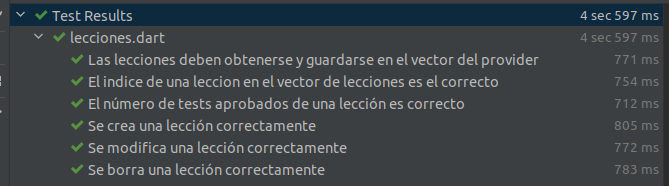
\includegraphics[width=\textwidth]{imagenes/c8/pruebalecciones.png}
    \caption{Resulados de las pruebas de unidad de las lecciones}
    \label{fig:pruebas_unidad_lecciones}
\end{figure}


\subsection{Preguntas}
\label{subsec:pruebas-unidad-preguntas}
Las pruebas realizadas sobre las preguntas son las siguientes:
\begin{itemize}
    \item \textbf{Obtención y guardado de preguntas del profesor}: Las preguntas de la vista del profesor deben obtenerse y guardarse en el vector del provider PreguntasProfesor (método fetchAndSetPreguntas). \textit{Después de ejecutar el método, el provider debe contener una lista no vacía de preguntas.}
    \item \textbf{Obtención del índice mediante el id}: Dado un id de una pregunta, se debe obtener el índice de la pregunta en el vector del provider (método getIndice). \textit{El método no debe devolver el valor '-1'.}
    \item \textbf{Creación de una pregunta}: Se debe crear una pregunta con los datos correctos (método crearPregunta). \textit{Tras ejecutar el método, el vector de preguntas del provider debe tener una longitud mayor que antes de ejecutarlo }
    \item \textbf{Modificación de una pregunta}: Se debe modificar una pregunta con los datos correctos (método modificarPregunta). \textit{Tras la ejución del método, los datos antiguos y nuevos de la pregunta deben ser distintos.}
    \item \textbf{Eliminación de una pregunta}: Se debe eliminar una pregunta coorectamente (método eliminarPregunta). \textit{Tras ejecutar el método, el provider no debe contener la pregunta.}
    \item \textbf{Obtención y guardado de preguntas}: Las preguntas deben obtenerse y guardarse en el vector del provider Preguntas (método fetchAndSetPreguntas). \textit{Después de ejecutar el método, el provider debe contener una lista no vacía de preguntas.}
    \item \textbf{Asignar opción}: Se debe asignar una opción a una pregunta correctamente cuando se crea o modifica una pregunta (método setValor). \textit{Tras ejecutar el método, las opciones de la pregunta deben coincidir con las opciones asignadas.}
    \item \textbf{Asignar respuesta}: Se debe asignar una respuesta a una pregunta correctamente cuando el usuario responde (método setRespuestas). \textit{Después de la ejecución, la respuesta de la pregunta debe coincidir con la respuesta asignada.}
    \item \textbf{Asignar pulsado}: Se debe asignar el valor de la variable "pulsado" correctamente cuando el usuario pulsa una opción (método setPulsado). \textit{Después de la ejecución, los valores del array "pulsado" deben coincidir con los asignados.}
\end{itemize}

\begin{figure}[H]
    \centering
    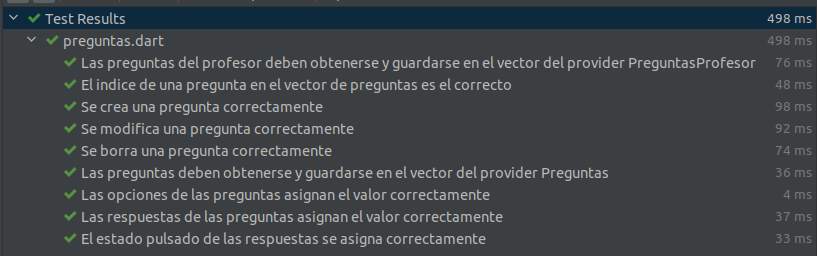
\includegraphics[width=\textwidth]{imagenes/c8/pruebapreguntas.png}
    \caption{Resulados de las pruebas de unidad de las preguntas}
    \label{fig:pruebas_unidad_preguntas}
\end{figure}


\subsection{Usuarios}
\label{subsec:pruebas-unidad-usuarios}
Las pruebas realizadas sobre los usuarios son las siguientes:
\begin{itemize}
    \item \textbf{Obtención y guardado}: Los usuarios deben obtenerse y guardarse en el vector del provider (método fetchAndSetUsuarios). \textit{Tras la ejecución del método el provider debe contener una lista no vacía de usuarios.}
    \item \textbf{Obtención del índice mediante el id}: Dado un id de un usuario, se debe obtener el índice del usuario en el vector del provider (método getIndice). \textit{El método no debe devolver el valor '-1'.}
    \item \textbf{Creación de un usuario}: Se debe crear un usuario con los datos correctos (método crearUsuario). \textit{Tras ejecutar el método, el vector de usuarios del provider debe tener una longitud mayor que antes de ejecutarlo.}
    \item \textbf{Modificación de un usuario}: Se debe modificar un usuario con los datos correctos (método modificarUsuario). \textit{Tras ejecutar el método, los datos antiguos y nuevos del usuario deben ser distintos.}
    \item \textbf{Eliminación de un usuario}: Se debe eliminar un usuario coorectamente (método eliminarUsuario). \textit{Tras ejecutar el método, el vector de usuarios del provider debe tener una longitud menor que antes de ejecutarlo.}
\end{itemize}

\begin{figure}[H]
    \centering
    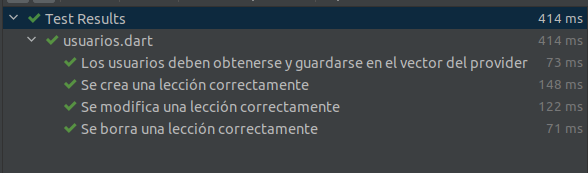
\includegraphics[width=\textwidth]{imagenes/c8/pruebausuarios.png}
    \caption{Resulados de las pruebas de unidad de los usuarios}
    \label{fig:pruebas_unidad_usuarios}
\end{figure}

\subsection{Logros}
\label{subsec:pruebas-unidad-logros}
Las pruebas realizadas sobre los logros son las siguientes:
\begin{itemize}
    \item \textbf{Obtención y guardado}: Los logros deben obtenerse y guardarse en el vector del provider (método fetchAndSetLogros). \textit{Tras la ejecución del método el provider debe contener una lista no vacía de logros.}
    \item \textbf{Obtención del índice mediante el id}: Dado un id de un logro, se debe obtener el índice del logro en el vector del provider (método getIndice). \textit{El método no debe devolver el valor '-1'.}
    \item \textbf{Creación de un logro}: Se debe crear un logro con los datos correctos (método crearLogro). \textit{Tras ejecutar el método, el vector de logros del provider debe tener una longitud mayor que antes de ejecutarlo.}
    \item \textbf{Modificación de un logro}: Se debe modificar un logro con los datos correctos (método modificarLogro). \textit{Tras ejecutar el método, los datos antiguos y nuevos del logro deben ser distintos.}
    \item \textbf{Eliminación de un logro}: Se debe eliminar un logro coorectamente (método borrarLogro). \textit{Tras ejecutar el método, el vector de logros del provider debe tener una longitud menor que antes de ejecutarlo.}
\end{itemize}

\begin{figure}[H]
    \centering
    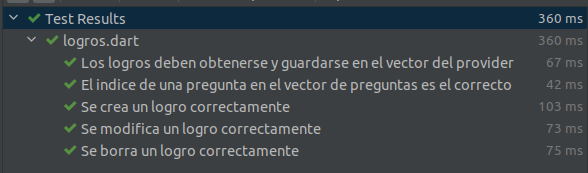
\includegraphics[width=\textwidth]{imagenes/c8/pruebalogros.png}
    \caption{Resulados de las pruebas de unidad de los logros}
    \label{fig:pruebas_unidad_logros}
\end{figure}


\section{Pruebas de controlador o widget}
\label{sec:pruebas-controlador}
Las pruebas de controlador o widget son aquellas que se realizan sobre los controladores o widgets de la aplicación (Figura \ref{fig:prueba_widgets}). Estas pruebas se realizan de forma individual, aislando el controlador o widget a probar de los demás componentes del sistema.
A continuación se muestran las pruebas realizadas sobre algunos widgets de la aplicación.

\subsection{Botón de inicio de sesión}
\label{subsec:pruebas-controlador-boton-inicio-sesión}
El botón de inicio de sesión se encuentra en la pantalla de inicio de la aplicación. Se ha realizado una prueba sobre el botón, comprobando que al pulsar el botón se accede a la pantalla de lecciones (pantalla principal de la aplicación).
El test verifica que al pulsar dicho botón aparece un texto perteneciente a la pantalla de lecciones, en este caso ``Los instrumentos''.

\subsection{Botón de acceso a lista de lecciones del profesor}
\label{subsec:pruebas-controlador-boton-lecciones}
El dashboard del usuario contiene un botón para acceder a las lecciones. Se ha realizado una prueba sobre el botón, comprobando que al pulsar el botón se accede a la pantalla de lista de lecciones. 
El test verifica que al pulsar dicho botón se muestra un texto perteneciente a la pantalla de lecciones, en este caso ``Crear Lección'' y ``Borrar''.

\subsection{Botón de acceso a lista de logros del profesor}
\label{subsec:pruebas-controlador-boton-logros}
El dashboard del usuario contiene un botón para acceder a los logros. Se ha realizado una prueba sobre el botón, comprobando que al pulsar el botón se accede a la pantalla de lista de logros. 
El test verifica que al pulsar dicho botón se muestra un texto perteneciente a la pantalla de logros, en este caso ``Crear Logro'' y ``Borrar'' (Figura \ref{fig:prueba_lista_logros}).
\begin{figure}[H]
    \centering
    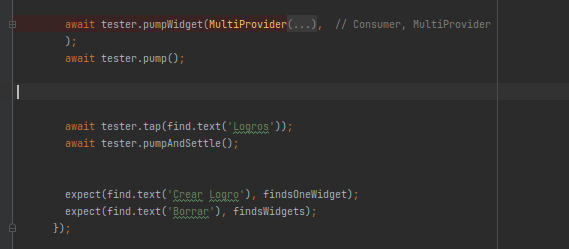
\includegraphics[width=\textwidth]{imagenes/c8/pruebawidget1.png}
    \caption{Código de la prueba de controlador o widget de acceso a lista de logros}
    \label{fig:prueba_lista_logros}
\end{figure}


\subsection{Botón de acceso a lista de preguntas del profesor}
\label{subsec:pruebas-controlador-boton-preguntas}
El dashboard del usuario contiene un botón para acceder a las preguntas. Se ha realizado una prueba sobre el botón, comprobando que al pulsar el botón se accede a la pantalla de lista de preguntas. 
El test verifica que al pulsar dicho botón aparece un texto perteneciente a la pantalla de preguntas, en este caso ``Crear Pregunta'' y ``Borrar''.

\subsection{Botón de acceso a lista de usuarios }
\label{subsec:pruebas-controlador-boton-usuarios}
El dashboard del usuario contiene un botón para acceder a los usuarios. Se ha realizado una prueba sobre el botón, comprobando que al pulsar el botón se accede a la pantalla de lista de usuarios. 
El test verifica que al pulsar dicho botón se muestra un texto perteneciente a la pantalla de usuarios, en este caso ``Crear Usuario'' y ``Borrar''.

\subsection{Botón de acceso al perfil del usuario}
\label{subsec:pruebas-controlador-boton-perfil-usuario}
El drawer contiene un botón para acceder al perfil del usuario. Se ha realizado una prueba sobre el botón, comprobando que al pulsar el botón se accede a la pantalla de perfil del usuario.
El test verifica que al pulsar dicho botón aparece un texto perteneciente a la pantalla de perfil del usuario, en este caso ``Mis logros''.

\subsection{Botón de acceso a una lección}
\label{subsec:pruebas-controlador-boton-leccion}
Al pulsar sobre una lección de la lista de lecciones, se accede a la pantalla de lección. Se ha realizado una prueba sobre el botón, comprobando que dicho acceso se realiza correctamente.
El test verifica que al pulsar dicho botón aparece un texto perteneciente a la pantalla de lección, en este caso ``Historial''.

\subsection{Botón de acceso al inicio}
\label{subsec:pruebas-controlador-boton-leccion}
El drawer contiene un botón para acceder a la pantalla de lecciones. Se ha realizado una prueba sobre el botón, comprobando que dicho acceso se realiza correctamente.
El test verifica que al pulsar dicho botón se muestra un texto perteneciente a la pantalla de lecciones, en este caso ``Los instrumentos'' (Figura \ref{fig:prueba_lecciones}).

\begin{figure}[H]
    \centering
    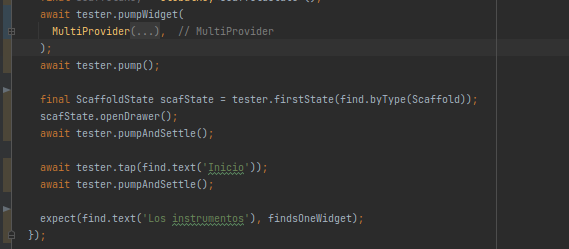
\includegraphics[width=\textwidth]{imagenes/c8/pruebawidget2.png}
    \caption{Código de la prueba de controlador o widget de acceso a la pantalla de lecciones}
    \label{fig:prueba_lecciones}
\end{figure}

\subsection{Botón de acceso al dashboard}
\label{subsec:pruebas-controlador-boton-leccion}
El drawer contiene un botón para acceder al dashboard. Se ha realizado una prueba sobre el botón, comprobando que dicho acceso se realiza correctamente.
El test verifica si al pulsar dicho botón encuentra un texto perteneciente a la pantalla de dashboard, en este caso ``Lecciones". 


\begin{figure}[H]
    \centering
    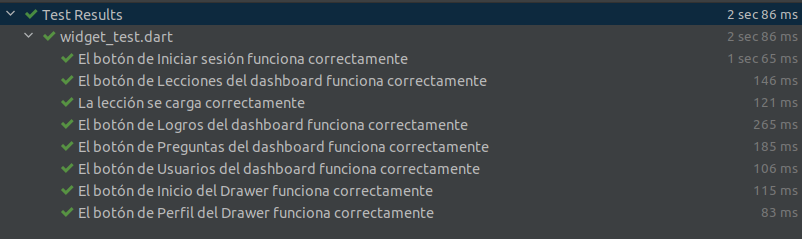
\includegraphics[width=\textwidth]{imagenes/c8/pruebawidgets.png}
    \caption{Resultados de las pruebas de controlador o widget}
    \label{fig:prueba_widgets}
\end{figure}


\section{Pruebas de sistema o de integración}
\label{sec:pruebas-sistema}
Las pruebas de sistema o de integración son aquellas que se realizan sobre el sistema completo. Estas pruebas tratan de verificar el flujo de uso de una determinada funcionalidad de la aplicación.
De esta forma nos aseguramos de que el sistema funciona de forma adecuada simulando varias acciones que podría realizar un usuario.

\subsection{Creación de usuario}
En este test se comprueba que se crea un usuario correctamente. Para ello se siguen los siguientes pasos:
\begin{enumerate}
    \item Se comienza en la pantalla de inicio de sesión.
    \item Se rellenan los campos de inicio de sesión con los datos del profesor.
    \item Se pulsa el botón de inicio de sesión.
    \item Se abre el drawer y se pulsa el botón de acceso a la dashboard.
    \item Se pulsa el botón de acceso a la gestión de Usuarios.
    \item Se pulsa el botón de crear usuario.
    \item Se rellenan los campos de creación de usuario con los datos del alumno.
    \item Se pulsa el botón de crear usuario.
    \item Se comprueba que se ha creado el usuario.
\end{enumerate}

\begin{figure}[H]
    \centering
    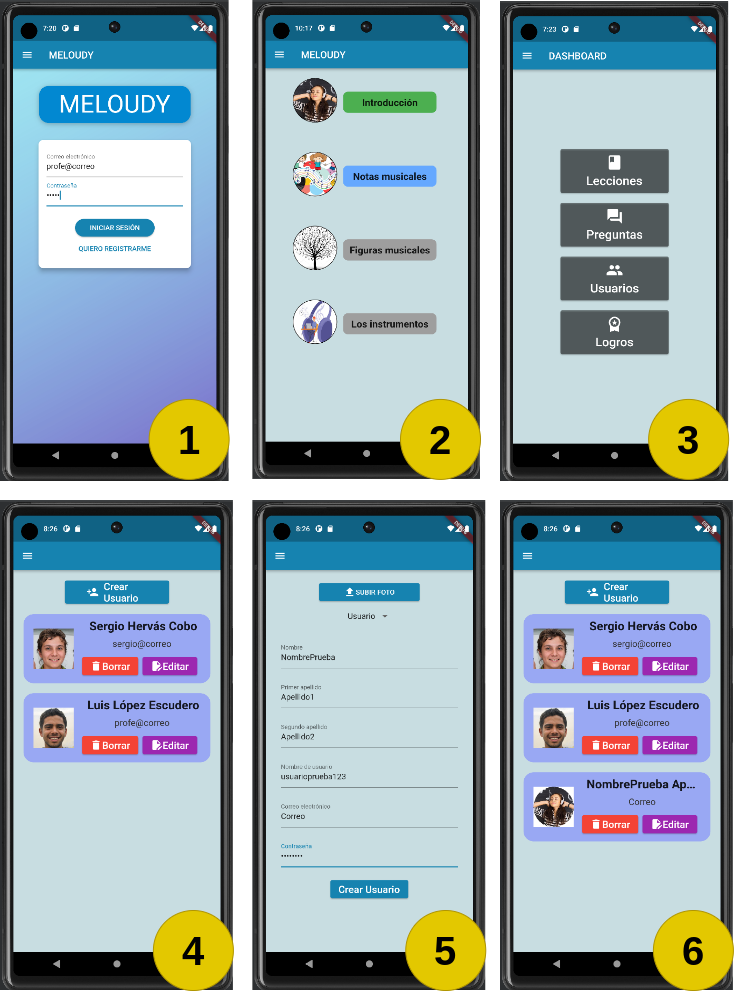
\includegraphics[width=\textwidth]{imagenes/c8/testint1.png}
    \caption{Pantallas por las que pasa la prueba de creación de usuario}
    \label{fig:prueba_creacion_usuario}
\end{figure}

\newpage


\subsection{Edición de datos del perfil}

\begin{figure}[H]
    \centering
    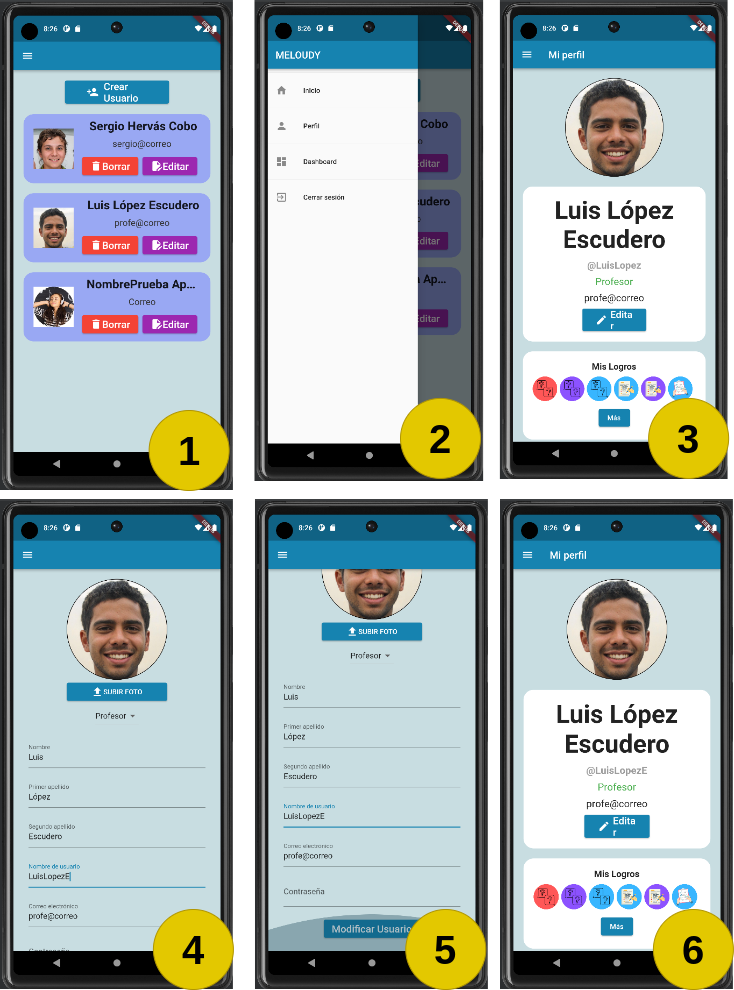
\includegraphics[width=\textwidth]{imagenes/c8/testint2.png}
    \caption{Pantallas por las que pasa la prueba de modificación de datos del perfil}
    \label{fig:prueba_edicion_perfil}
\end{figure}

Esta prueba verifica que se editen los datos del perfil de un usuario (Figura \ref{fig:prueba_edicion_perfil}). Para ello se siguen los siguientes pasos:

\begin{enumerate}
    \item Se comienza en la pantalla de lista de lecciones. (la sesión ya está iniciada del test anterior)
    \item Se abre el drawer y se pulsa el botón de acceso al perfil del usuario.
    \item Se pulsa el botón de editar perfil.
    \item Se rellenan los campos de edición de perfil con los nuevos datos del profesor.
    \item Se pulsa el botón de editar perfil.
    \item Se comprueba que se han editado los datos del perfil.
\end{enumerate}



\subsection{Realización de un test}
Esta prueba verifica que se puede realizar un test (Figura \ref{fig:prueba_realizacion_test}) y contestar a las preguntas de este. Para ello se siguen los siguientes pasos:
\begin{enumerate}
    \item Se comienza en la pantalla de lista de lecciones.
    \item Se pulsa sobre la lección "Introducción" (por ejemplo).
    \item Se pulsa el botón de "Hacer Test".
    \item Se responde a las preguntas en función del tipo:
    \begin{enumerate}
        \item Si es de tipo "unica", se pulsa sobre la segunda opción.
        \item Si es de tipo "multiple", se pulsa sobre la segunda y la tercera opción.
        \item Si es de tipo "texto", se escribe una respuesta cualquiera. En este caso se ha escrito "melodía".
    \end{enumerate}
    \item Se pulsa el botón de "Enviar".
    \item Se comprueba que se ha realizado el test.
\end{enumerate}

\begin{figure}[H]
    \centering
    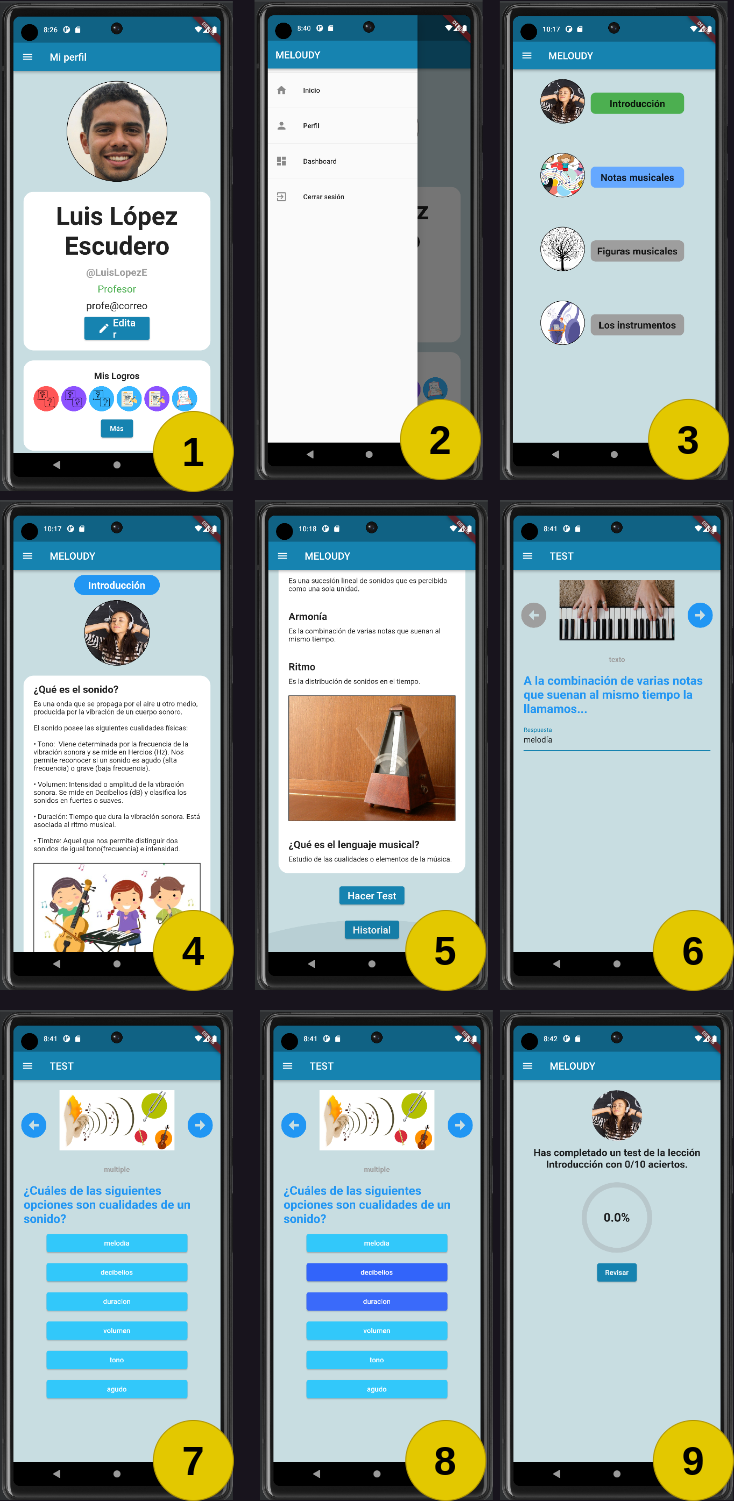
\includegraphics[width=0.85\textwidth]{imagenes/c8/testint3.png}
    \caption{Pantallas por las que pasa la prueba de realización de un test}
    \label{fig:prueba_realizacion_test}
\end{figure}
